\documentclass[11pt,oneside]{article}

\usepackage[T1]{fontenc}
\usepackage[utf8]{inputenc}
\usepackage{lmodern}
\usepackage{microtype}
\usepackage[margin=1in]{geometry}
\usepackage{amsmath,amssymb,amsthm,mathtools}
\usepackage{mathrsfs}
\usepackage{bm}
\usepackage{booktabs,longtable,array}
\usepackage{enumitem}
\usepackage{xcolor}
\usepackage{tikz}
\usetikzlibrary{arrows.meta,calc,decorations.pathreplacing,positioning}
\usepackage[most]{tcolorbox}
\usepackage{listings}
\usepackage{xurl}
\usepackage{hyperref}
\usepackage[nameinlink,noabbrev]{cleveref}

\definecolor{DeepBlue}{HTML}{17365D}
\definecolor{AccentBlue}{HTML}{2A6F97}
\definecolor{PaleBlue}{HTML}{EEF6FB}
\definecolor{PaleGold}{HTML}{FFF8E8}
\definecolor{DeepGold}{HTML}{8A5A00}
\definecolor{PaleGray}{HTML}{F5F6F7}
\definecolor{CodeGray}{HTML}{F7F7F7}

\hypersetup{
  colorlinks=true,
  linkcolor=DeepBlue,
  citecolor=AccentBlue,
  urlcolor=AccentBlue,
  pdftitle={Exact Pole-Lattice Transseries for the Fubini Numbers},
  pdfauthor={Research article prepared for Vladimir Reshetnikov},
  pdfsubject={Ordered Bell numbers, asymptotic transseries, pole lattice, coefficient calculus},
  pdfkeywords={Fubini numbers, ordered Bell numbers, transseries, asymptotics, Stirling coefficients, Bell polynomials}
}

\setlength{\parindent}{0pt}
\setlength{\parskip}{0.55em}
\setlist[itemize]{leftmargin=2em,itemsep=0.25em,topsep=0.25em}
\setlist[enumerate]{leftmargin=2.2em,itemsep=0.25em,topsep=0.25em}
\allowdisplaybreaks[3]
\numberwithin{equation}{section}

\newtheorem{theorem}{Theorem}[section]
\newtheorem{proposition}[theorem]{Proposition}
\newtheorem{lemma}[theorem]{Lemma}
\newtheorem{corollary}[theorem]{Corollary}
\newtheorem{definition}[theorem]{Definition}
\newtheorem{remark}[theorem]{Remark}
\newtheorem{example}[theorem]{Example}

\newtcolorbox{mainbox}[1][]{
  enhanced,breakable,colback=PaleBlue,colframe=AccentBlue,
  boxrule=0.9pt,arc=2pt,left=8pt,right=8pt,top=7pt,bottom=7pt,
  title={#1},fonttitle=\bfseries,coltitle=DeepBlue
}
\newtcolorbox{auditbox}[1][]{
  enhanced,breakable,colback=PaleGold,colframe=DeepGold,
  boxrule=0.8pt,arc=2pt,left=8pt,right=8pt,top=7pt,bottom=7pt,
  title={#1},fonttitle=\bfseries,coltitle=DeepGold
}
\newtcolorbox{notebox}[1][]{
  enhanced,breakable,colback=PaleGray,colframe=black!45,
  boxrule=0.6pt,arc=2pt,left=8pt,right=8pt,top=6pt,bottom=6pt,
  title={#1},fonttitle=\bfseries
}

\lstdefinestyle{code}{
  backgroundcolor=\color{CodeGray},
  basicstyle=\ttfamily\small,
  frame=single,
  rulecolor=\color{black!25},
  breaklines=true,
  columns=fullflexible,
  keepspaces=true,
  showstringspaces=false,
  xleftmargin=0.5em,
  xrightmargin=0.5em,
  aboveskip=0.8em,
  belowskip=0.8em
}
\lstset{style=code}

\newcommand{\e}{\mathrm e}
\newcommand{\ii}{\mathrm i}
\newcommand{\dd}{\,\mathrm d}
\newcommand{\N}{\mathbb N}
\newcommand{\Z}{\mathbb Z}
\newcommand{\C}{\mathbb C}
\newcommand{\R}{\mathbb R}
\newcommand{\Fub}{\mathsf F}
\newcommand{\Log}{\operatorname{Log}}
\newcommand{\Li}{\operatorname{Li}}
\newcommand{\Res}{\operatorname*{Res}}
\newcommand{\Coeff}[2]{[#1^{#2}]}
\newcommand{\StirlingTwo}[2]{\left\{\!\begin{matrix}#1\\#2\end{matrix}\!\right\}}
\newcommand{\falling}[2]{(#1)_{\underline{#2}}}
\newcommand{\rising}[2]{(#1)_{\overline{#2}}}
\newcommand{\abs}[1]{\left|#1\right|}
\newcommand{\norm}[1]{\left\lVert#1\right\rVert}
\newcommand{\paren}[1]{\left(#1\right)}
\newcommand{\bracket}[1]{\left[#1\right]}
\newcommand{\set}[1]{\left\{#1\right\}}
\newcommand{\sym}{\mathrm{sym}}
\newcommand{\supp}{\operatorname{supp}}
\newcommand{\RePart}{\operatorname{Re}}
\newcommand{\ImPart}{\operatorname{Im}}

\crefname{equation}{equation}{equations}
\Crefname{equation}{Equation}{Equations}
\crefname{section}{section}{sections}
\Crefname{section}{Section}{Sections}

\begin{document}
\hypersetup{pageanchor=false}

\begin{titlepage}
\centering
\vspace*{1.2cm}
{\color{DeepBlue}\rule{0.92\textwidth}{1.2pt}}\\[1.25cm]
{\Huge\bfseries Exact Pole--Lattice Transseries\\[0.2em]
for the Fubini Numbers\par}
\vspace{0.55cm}
{\Large Complete exponential corrections, general coefficient formulae,\\
rigorous remainder bounds, and nonlinear sector calculus\par}
\vspace{1.1cm}
{\color{DeepBlue}\rule{0.72\textwidth}{0.7pt}}\\[1.1cm]
{\large Research article prepared for Vladimir Reshetnikov\par}
\vspace{0.3cm}
{\large 3 September 2026\par}
\vfill
\begin{minipage}{0.86\textwidth}
\small
\textbf{Scope.} The ordered Bell (Fubini) numbers have a meromorphic exponential generating function with an infinite vertical lattice of simple poles.  Exploiting the complete Mittag--Leffler decomposition gives an exact, absolutely convergent transseries after factorial normalization.  This article derives that representation, resolves every exponentially small conjugate-pole sector, gives closed formulae for every algebraic coefficient under Stirling normalization, proves explicit truncation estimates, and develops the induced coefficient calculus for logarithms, powers, reciprocals, ratios, and the Fubini polynomials.
\end{minipage}
\vfill
{\color{DeepBlue}\rule{0.92\textwidth}{1.2pt}}
\end{titlepage}
\hypersetup{pageanchor=true}
\pagenumbering{roman}

\begin{abstract}
Let \(\Fub_n=\sum_{j=0}^n j!\StirlingTwo{n}{j}\) be the \(n\)-th Fubini number, and put \(\rho=\log 2\), \(N=n+1\), and \(\rho_k=\rho+2\pi\ii k\).  We prove the exact identity
\[
 \Fub_n=\frac{\Gamma(N)}{2}\sum_{k\in\Z}\rho_k^{-N}
       =\frac{\Gamma(N)}{2\rho^N}\sum_{k\in\Z}\e^{-N\Omega_k},
 \qquad
 \Omega_k=\Log\!\paren{1+\frac{2\pi\ii k}{\rho}},
\]
valid for every integer \(n\ge1\).  The sum converges absolutely and is not merely asymptotic.  Pairing conjugate poles gives the exact real oscillatory transseries
\[
 \Fub_n=\frac{n!}{2\rho^{n+1}}
 \left[1+2\sum_{k\ge1}\e^{-(n+1)\mu_k}
 \cos\!\bigl((n+1)\theta_k\bigr)\right],
\]
where \(\mu_k=\tfrac12\log(1+(2\pi k/\rho)^2)\) and
\(\theta_k=\arctan(2\pi k/\rho)\).  We give a sharp sector ordering and explicit Hurwitz-zeta and first-omitted-scale bounds for every finite pole truncation.

After replacing \(\Gamma(N)\) by its Stirling expansion, the complete two-index coefficient array factorizes: the coefficient in every pole sector is the same Stirling coefficient \(g_m\).  These coefficients are determined equivalently by a Bernoulli-number generating function, a partition sum over odd parts, a complete exponential Bell polynomial, and a triangular recurrence.  In the exact-factorial normalization the stronger statement holds: each pole sector has coefficient \(1\) at algebraic order zero and all higher algebraic coefficients vanish.  Finally, a countable-variable multinomial theorem gives general coefficients for analytic functions of the normalized transseries, including explicit multi-sector formulae for \(\log \Fub_n\), arbitrary powers, reciprocals, and shifted ratios.  The entire construction extends verbatim to Fubini polynomials and geometric moments.
\end{abstract}

\begin{mainbox}[Principal result at a glance]
For \(n\ge1\), set \(N=n+1\), \(\rho=\log2\), and
\[
 \Omega_k=\mu_{|k|}+\ii\,\operatorname{sgn}(k)\theta_{|k|}
 =\Log\!\paren{1+\frac{2\pi\ii k}{\rho}},\qquad \Omega_0=0.
\]
Then
\begin{align*}
 \frac{2\rho^N\Fub_{N-1}}{\Gamma(N)}
 &=\sum_{k\in\Z}\e^{-N\Omega_k}\\
 &=1+2\sum_{k\ge1}\e^{-N\mu_k}\cos(N\theta_k),
\end{align*}
\emph{exactly}.  If \(K\ge0\), the omitted tail satisfies
\[
 \abs{R_{K,N}}
 \le 2\paren{\frac{\rho}{2\pi}}^N\zeta(N,K+1),
\]
with the convention that \(\zeta(N,1)=\zeta(N)\).  Under the elementary prefactor
\[
 P_N=\frac{\sqrt{2\pi}}{2}\,N^{N-1/2}\e^{-N}\rho^{-N},
\]
the full formal coefficient array is
\[
 \Fub_{N-1}\sim P_N
 \sum_{k\in\Z}\sum_{m\ge0}g_mN^{-m}\e^{-N\Omega_k},
 \qquad c_{k,m}=g_m,
\]
where
\[
 \sum_{m\ge0}g_mt^m
 =\exp\!\left(\sum_{j\ge1}\frac{\beta_{2j}}{2j(2j-1)}t^{2j-1}\right).
\]
Here \(\beta_j\) are Bernoulli numbers, defined by
\(t/(\e^t-1)=\sum_{j\ge0}\beta_jt^j/j!\).
\end{mainbox}

\tableofcontents
\newpage
\pagenumbering{arabic}

\section{Introduction}

\subsection{Why the Fubini case is unusually rigid}

The Fubini numbers, also called \emph{ordered Bell numbers} or \emph{preferential-arrangement numbers}, count ordered set partitions.  Their first values are
\[
 1,\ 1,\ 3,\ 13,\ 75,\ 541,\ 4683,\ 47293,\ 545835,\ldots.
\]
They look superficially similar to the ordinary Bell numbers, but their asymptotic mechanisms are fundamentally different.  The ordinary Bell exponential generating function is entire, and its coefficients are governed by a moving saddle involving Lambert's \(W\)-function.  The Fubini generating function
\[
 \mathcal F(z)=\frac{1}{2-\e^z}
\]
is meromorphic.  Its singularities are the equally spaced simple poles
\[
 \rho_k=\log2+2\pi\ii k,\qquad k\in\Z.
\]
The nearest pole \(\rho_0=\log2\) gives the classical leading approximation.  Every remaining pole gives an exponentially smaller oscillatory correction.  Because all poles are simple and all residues are the same, the complete correction hierarchy is much more rigid than a generic saddle-point or algebraic-singularity expansion.

The principal observation of this article is stronger still.  A Mittag--Leffler decomposition of \(1/(2-\e^z)\) has only a \emph{constant} entire correction.  Consequently, every Taylor coefficient of positive degree is exactly the sum of the principal-part contributions of all poles.  The resulting pole expansion is therefore simultaneously
\begin{itemize}
 \item an exact convergent representation;
 \item a complete exponentially ordered transseries;
 \item an exponentially improved singularity-analysis expansion; and
 \item a particularly simple example of oscillatory conjugate-action bookkeeping.
\end{itemize}

\subsection{Relation to the supplied research framework}

The linked \emph{Combinatorial Coefficient Calculus} develops ordered Bell numbers from labelled set partitions, Stirling numbers of the second kind, and exponential generating functions, with particular care about coefficient conventions and the distinction among Bell, Bernoulli, and Bell-polynomial notation.  The linked series-and-transseries material emphasizes asymptotically ordered sectors, conjugate complex actions, and residual or remainder certificates.  The present article joins these two viewpoints: the pole lattice provides the actions, while Bernoulli numbers and complete exponential Bell polynomials provide the algebraic coefficients.

The exact pole identity itself is classical in substance; it can be obtained from Mittag--Leffler expansion or Poisson summation.  The contribution here is a systematic and fully normalized transseries formulation, including all sectors, all coefficient formulae, explicit truncation bounds, nonlinear action-semigroup calculus, and a parameterized extension.

\begin{auditbox}[Meaning of ``full'' in this article]
The word \emph{full} refers to the complete hierarchy generated by every singularity of the Fubini exponential generating function, with the factorial \(\Gamma(N)\) retained exactly.  In this normalization the transseries is itself exact.  When \(\Gamma(N)\) is subsequently replaced by its elementary Stirling expansion, one obtains a formal algebraic layer with coefficients \(g_m\).  Hyperasymptotic completion of the Stirling series for \(\Gamma\) is the standard, independent Gamma-function problem; it is not a missing Fubini pole sector.  Retaining \(\Gamma(N)\) exactly cleanly separates these two issues.
\end{auditbox}

\subsection{Organization}

\Cref{sec:combinatorial} establishes the combinatorial and generating-function identities.  \Cref{sec:poles} derives the exact pole sum.  \Cref{sec:transseries} constructs and orders the complete oscillatory transseries and proves remainder estimates.  \Cref{sec:coefficients} develops the Stirling coefficient calculus.  \Cref{sec:nonlinear} gives general multi-sector coefficients for nonlinear observables.  \Cref{sec:polynomials} extends the construction to Fubini polynomials and geometric moments.  \Cref{sec:numerics} supplies numerical checks and algorithms.  The appendices give a Poisson-summation proof, a continuous polylogarithmic interpolation, and an extended coefficient table.

\section{Combinatorial and generating-function foundations}
\label{sec:combinatorial}

\subsection{Ordered set partitions}

Let \(\StirlingTwo{n}{j}\) denote a Stirling number of the second kind.  It counts partitions of an \(n\)-element labelled set into \(j\) nonempty, unordered blocks.  Ordering the \(j\) blocks in \(j!\) ways gives the Fubini number
\begin{equation}
 \Fub_n=\sum_{j=0}^{n}j!\StirlingTwo{n}{j},
 \qquad n\ge0.
 \label{eq:fubini-stirling}
\end{equation}
We take \(\Fub_0=1\), corresponding to the unique empty ordered partition.

A first-block decomposition gives, for \(n\ge1\),
\begin{equation}
 \Fub_n=\sum_{j=1}^{n}\binom{n}{j}\Fub_{n-j}
       =\sum_{r=0}^{n-1}\binom{n}{r}\Fub_r.
 \label{eq:fubini-recurrence}
\end{equation}
Indeed, choose the nonempty first block and then order-partition its complement.

\subsection{Exponential generating function}

The standard exponential generating function for a fixed number of blocks is
\[
 \sum_{n\ge0}\StirlingTwo{n}{j}\frac{z^n}{n!}
 =\frac{(\e^z-1)^j}{j!}.
\]
Multiplying by \(j!\), summing over \(j\), and working first formally gives
\begin{align}
 \mathcal F(z)
 :=\sum_{n\ge0}\Fub_n\frac{z^n}{n!}
 &=\sum_{j\ge0}(\e^z-1)^j
 =\frac{1}{2-\e^z}.
 \label{eq:fubini-egf}
\end{align}
Analytically, the geometric sum is valid near \(z=0\), and the resulting meromorphic function provides the continuation.

\subsection{A geometric-moment or Dobiński-type formula}

Expanding \(\mathcal F\) in a different geometric series gives
\begin{align}
 \mathcal F(z)
 &=\frac12\frac{1}{1-\e^z/2}
 =\frac12\sum_{m\ge0}\frac{\e^{mz}}{2^m}.
 \label{eq:geometric-egf-expansion}
\end{align}
Termwise coefficient extraction yields
\begin{equation}
 \boxed{\displaystyle
 \Fub_n=\frac12\sum_{m\ge0}\frac{m^n}{2^m}}
 \qquad(n\ge0),
 \label{eq:fubini-dobinski}
\end{equation}
with the conventional value \(0^0=1\).  Thus \(\Fub_n\) is the \(n\)-th raw moment of a geometric random variable on \(\N_0\) with mass \(2^{-m-1}\).

The identities \cref{eq:fubini-stirling,eq:fubini-egf,eq:fubini-dobinski} are three coordinate systems for the same sequence: finite Stirling transform, meromorphic exponential generating function, and geometric moment sum.  The pole-lattice transseries will connect the last two by Fourier analysis or Mittag--Leffler expansion.

\section{The pole lattice and an exact coefficient formula}
\label{sec:poles}

\subsection{Location and residues of the singularities}

Put
\begin{equation}
 \rho:=\log2,
 \qquad
 \rho_k:=\rho+2\pi\ii k,
 \qquad k\in\Z.
 \label{eq:rho-definitions}
\end{equation}
The zeros of \(2-\e^z\) are precisely the \(\rho_k\).  Since
\[
 \frac{\dd}{\dd z}(2-\e^z)\bigg|_{z=\rho_k}=-\e^{\rho_k}=-2,
\]
every pole is simple and
\begin{equation}
 \Res_{z=\rho_k}\mathcal F(z)=-\frac12.
 \label{eq:residue}
\end{equation}
Writing \(w=z-\rho_k\), the local Laurent expansion is
\begin{equation}
 \mathcal F(\rho_k+w)
 =-\frac{1}{2w}+\frac14-\frac{w}{24}
 +\frac{w^3}{1440}-\frac{w^5}{60480}+\cdots.
 \label{eq:local-laurent}
\end{equation}
Only the principal part is singular.  Its coefficient contribution is
\begin{equation}
 \Coeff{z}{n}\paren{-\frac{1}{2(z-\rho_k)}}
 =\frac{1}{2\rho_k^{n+1}}.
 \label{eq:single-pole-coefficient}
\end{equation}

\subsection{Mittag--Leffler decomposition}

We use the classical symmetric partial-fraction identity
\begin{equation}
 \frac{1}{\e^w-1}
 =\frac1w-\frac12
 +2w\sum_{k=1}^{\infty}\frac{1}{w^2+4\pi^2k^2},
 \label{eq:bernoulli-mittag}
\end{equation}
valid locally uniformly away from \(2\pi\ii\Z\).  Since
\(\mathcal F(z)=-\tfrac12(\e^{z-\rho}-1)^{-1}\), this becomes
\begin{align}
 \mathcal F(z)
 &=\frac14-\frac12\left[
 \frac{1}{z-\rho}
 +\sum_{k=1}^{\infty}
 \left(\frac{1}{z-\rho-2\pi\ii k}
      +\frac{1}{z-\rho+2\pi\ii k}\right)
 \right]
 \notag\\
 &=\frac14-\frac12\sum_{k\in\Z}^{\sym}\frac{1}{z-\rho_k}.
 \label{eq:fubini-mittag}
\end{align}
The superscript \(\sym\) means symmetric summation in \(k\).  Pairing \(k\) and \(-k\) makes the summand \(O(k^{-2})\), so the displayed meromorphic series converges locally uniformly away from its poles.

The entire correction in \cref{eq:fubini-mittag} is the constant \(1/4\).  This fact is exactly what makes the positive-degree coefficient formula a pure sum of pole principal parts.

\begin{theorem}[Exact pole formula]
\label{thm:exact-pole-formula}
For every integer \(n\ge1\), with \(N=n+1\),
\begin{equation}
 \boxed{\displaystyle
 \Fub_n=\frac{\Gamma(N)}{2}
 \sum_{k\in\Z}(\rho+2\pi\ii k)^{-N}.}
 \label{eq:exact-pole-formula}
\end{equation}
The series is absolutely convergent.
\end{theorem}

\begin{proof}
Extract the coefficient of \(z^n\) from \cref{eq:fubini-mittag}.  The constant \(1/4\) contributes nothing because \(n\ge1\).  For each \(k\), \cref{eq:single-pole-coefficient} gives \(1/(2\rho_k^{n+1})\).  Moreover,
\[
 \sum_{k\in\Z}\abs{\rho_k}^{-N}<\infty
 \qquad(N\ge2),
\]
so coefficient extraction may be interchanged with summation.  Finally, \(\Fub_n/n!=\Coeff{z}{n}\mathcal F(z)\), and \(n!=\Gamma(N)\).
\end{proof}

\begin{remark}[The exceptional constant coefficient]
The formula is deliberately stated for \(n\ge1\).  At \(n=0\), symmetric summation gives
\[
 \frac12\sum_{k\in\Z}^{\sym}\rho_k^{-1}=\frac34,
\]
and the omitted Mittag--Leffler constant \(1/4\) restores \(\Fub_0=1\).  No such correction occurs in positive degree.
\end{remark}

\subsection{Geometric picture}

\begin{figure}[ht]
\centering
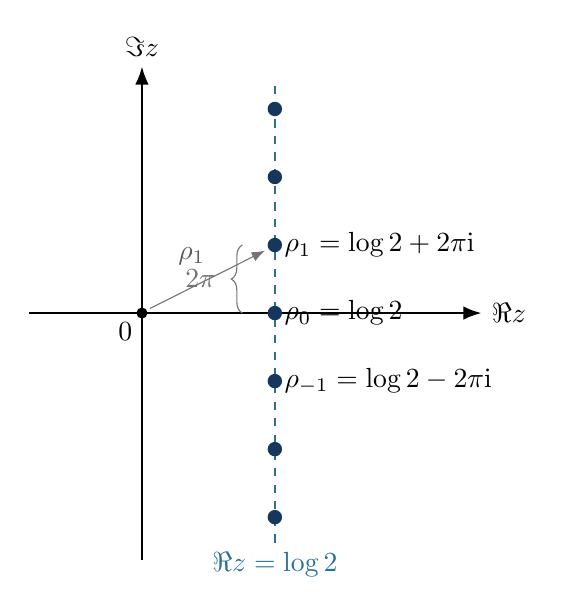
\begin{tikzpicture}[x=1.25cm,y=0.72cm,>=Latex]
  \draw[->,thick] (-1.15,0)--(3.45,0) node[right] {$\Re z$};
  \draw[->,thick] (0,-4.35)--(0,4.35) node[above] {$\Im z$};
  \draw[dashed,AccentBlue,thick] (1.35,-4.05)--(1.35,4.05);
  \fill (0,0) circle (2pt) node[below left] {$0$};
  \foreach \j/\y in {-3/-3.6,-2/-2.4,-1/-1.2,0/0,1/1.2,2/2.4,3/3.6}{
    \fill[DeepBlue] (1.35,\y) circle (2.6pt);
  }
  \node[right] at (1.35,0) {$\rho_0=\log2$};
  \node[right] at (1.35,1.2) {$\rho_1=\log2+2\pi\ii$};
  \node[right] at (1.35,-1.2) {$\rho_{-1}=\log2-2\pi\ii$};
  \node[below,AccentBlue] at (1.35,-4.05) {$\Re z=\log2$};
  \draw[->,black!55] (0.08,0.08)--(1.25,1.1);
  \node[above left,black!65] at (0.74,0.68) {$\rho_1$};
  \draw[decorate,decoration={brace,amplitude=4pt},black!55]
      (1.02,0)--(1.02,1.2) node[midway,left=6pt] {$2\pi$};
\end{tikzpicture}
\caption{The poles of \(1/(2-\e^z)\) form a vertical lattice.  Their moduli increase with \(\abs{k}\), so their coefficient contributions form an exponentially ordered hierarchy.}
\label{fig:pole-lattice}
\end{figure}

\section{The exact oscillatory transseries}
\label{sec:transseries}

\subsection{Actions, decay rates, and phases}

For \(k\in\Z\), define the complex action
\begin{equation}
 \Omega_k:=\Log\!\paren{\frac{\rho_k}{\rho}}
 =\Log\!\paren{1+\frac{2\pi\ii k}{\rho}},
 \qquad \Omega_0=0,
 \label{eq:action-definition}
\end{equation}
where \(\Log\) is the principal logarithm.  For \(k\ge1\), write
\begin{align}
 r_k&:=\abs{\rho_k}=\sqrt{\rho^2+4\pi^2k^2},
 \label{eq:rk}\\
 \lambda_k&:=\frac{\rho}{r_k}
 =\paren{1+\frac{4\pi^2k^2}{\rho^2}}^{-1/2},
 \label{eq:lambdak}\\
 \mu_k&:=-\log\lambda_k
 =\frac12\log\!\paren{1+\frac{4\pi^2k^2}{\rho^2}},
 \label{eq:muk}\\
 \theta_k&:=\arctan\!\paren{\frac{2\pi k}{\rho}}.
 \label{eq:thetak}
\end{align}
Then
\begin{equation}
 \Omega_{\pm k}=\mu_k\pm\ii\theta_k,
 \qquad
 \e^{-N\Omega_{\pm k}}
 =\lambda_k^N\e^{\mp\ii N\theta_k}.
 \label{eq:action-polar}
\end{equation}
The decay rates satisfy
\[
 0<\mu_1<\mu_2<\mu_3<\cdots,
\]
so the sectors are canonically ordered by \(\abs{k}\).

\subsection{Exact complex and real forms}

\begin{theorem}[Exact full pole-lattice transseries]
\label{thm:exact-transseries}
For every integer \(n\ge1\), with \(N=n+1\),
\begin{align}
 \mathscr T_N
 :=\frac{2\rho^N\Fub_{N-1}}{\Gamma(N)}
 &=\sum_{k\in\Z}\e^{-N\Omega_k}
 \label{eq:exact-complex-transseries}\\
 &=1+2\sum_{k=1}^{\infty}
 \e^{-N\mu_k}\cos(N\theta_k).
 \label{eq:exact-real-transseries}
\end{align}
Both series are absolutely convergent.  Thus \cref{eq:exact-complex-transseries,eq:exact-real-transseries} are exact identities, not only formal asymptotic statements.
\end{theorem}

\begin{proof}
Factor \(\rho^{-N}\) from \cref{eq:exact-pole-formula} and use
\[
 \paren{\frac{\rho}{\rho_k}}^N=\e^{-N\Omega_k}.
\]
Absolute convergence follows from \(\abs{\rho_k}^{-N}=O(\abs{k}^{-N})\), since \(N\ge2\).  Pairing \(k\) with \(-k\) and using \cref{eq:action-polar} gives the real form.
\end{proof}

\begin{definition}[Sector truncation]
For \(K\ge0\), define
\begin{align}
 \mathscr T_N^{[K]}
 &:=\sum_{\abs{k}\le K}\e^{-N\Omega_k}
 =1+2\sum_{k=1}^{K}\e^{-N\mu_k}\cos(N\theta_k),
 \label{eq:sector-truncation}\\
 R_{K,N}&:=\mathscr T_N-\mathscr T_N^{[K]}.
 \label{eq:sector-remainder}
\end{align}
When \(K=0\), the approximation keeps only the dominant real pole.
\end{definition}

\subsection{Explicit tail bounds}

\begin{theorem}[Hurwitz-zeta bound]
\label{thm:hurwitz-bound}
For \(N\ge2\) and \(K\ge0\),
\begin{equation}
 \boxed{\displaystyle
 \abs{R_{K,N}}
 \le 2\paren{\frac{\rho}{2\pi}}^N\zeta(N,K+1),}
 \label{eq:hurwitz-tail-bound}
\end{equation}
where \(\zeta(s,a)=\sum_{j=0}^{\infty}(j+a)^{-s}\) is the Hurwitz zeta function.  In particular,
\begin{equation}
 \abs{\mathscr T_N-1}
 \le 2\paren{\frac{\rho}{2\pi}}^N\zeta(N).
 \label{eq:dominant-tail-bound}
\end{equation}
For \(N\ge2\), the right side of \cref{eq:dominant-tail-bound} is at most
\(0.040038\).
\end{theorem}

\begin{proof}
By the triangle inequality and \(r_k\ge2\pi k\),
\begin{align*}
 \abs{R_{K,N}}
 &\le2\sum_{k=K+1}^{\infty}\lambda_k^N
 =2\sum_{k=K+1}^{\infty}
   \paren{\frac{\rho}{\sqrt{\rho^2+4\pi^2k^2}}}^{N}\\
 &\le2\paren{\frac{\rho}{2\pi}}^N
   \sum_{k=K+1}^{\infty}k^{-N},
\end{align*}
which is \cref{eq:hurwitz-tail-bound}.  At \(N=2\), the bound in
\cref{eq:dominant-tail-bound} equals
\(2(\rho/(2\pi))^2\zeta(2)=0.0400377511\ldots\); it decreases thereafter because both \((\rho/(2\pi))^N\) and \(\zeta(N)\) decrease.
\end{proof}

The Hurwitz-zeta estimate is simple and uniform, although its exponential rate is slightly weaker than the exact first-omitted-pole rate.  The latter is recovered as follows.

\begin{proposition}[Sharp first-omitted-scale ordering]
\label{prop:sharp-ordering}
For each fixed \(K\ge0\),
\begin{equation}
 R_{K,N}=2\e^{-N\mu_{K+1}}\cos(N\theta_{K+1})
 +O_K\!\paren{\e^{-N\mu_{K+2}}}
 \qquad(N\to\infty).
 \label{eq:first-omitted-pair}
\end{equation}
In particular,
\begin{equation}
 R_{K,N}=O_K\!\paren{\e^{-N\mu_{K+1}}}.
 \label{eq:sharp-big-o}
\end{equation}
\end{proposition}

\begin{proof}
Separate the pair \(k=\pm(K+1)\).  For the remaining tail, factor out \(\lambda_{K+2}^N\):
\[
 \sum_{k=K+2}^{\infty}\lambda_k^N
 =\lambda_{K+2}^N
  \sum_{k=K+2}^{\infty}\paren{\frac{r_{K+2}}{r_k}}^N.
\]
For \(N\ge2\), the sum is bounded by
\(\sum_{k=K+2}^{\infty}(r_{K+2}/r_k)^2<\infty\), independently of \(N\).  This proves \cref{eq:first-omitted-pair}; \cref{eq:sharp-big-o} follows by the same argument without first separating the pair.
\end{proof}

\subsection{Leading and exponentially improved asymptotics}

The dominant pole gives
\begin{equation}
 \Fub_n\sim\frac{n!}{2(\log2)^{n+1}}.
 \label{eq:classical-leading}
\end{equation}
The complete nearest-pair improvement is
\begin{equation}
 \Fub_n=\frac{n!}{2\rho^{n+1}}
 \left[1+2\lambda_1^{n+1}
 \cos\!\bigl((n+1)\theta_1\bigr)
 +O\!\paren{\lambda_2^{n+1}}\right].
 \label{eq:first-exponential-improvement}
\end{equation}
Numerically,
\begin{align}
 \lambda_1&=0.109652580999385\ldots,
 &\mu_1&=2.210438265869183\ldots,
 &\theta_1&=1.460922810208262\ldots.
 \label{eq:first-action-numerics}
\end{align}
Hence the relative error of the dominant-pole approximation is not merely algebraically small; it is an oscillatory quantity of order roughly \(0.10965^{n+1}\).

Because the cosine can be close to zero for individual \(n\), the numerical error may occasionally be much smaller than the nominal first-sector envelope.  The complex form \cref{eq:exact-complex-transseries}, rather than the paired cosine form, is the cancellation-free statement of the sector ordering.

\subsection{Why each exact sector is flat}

A generic singularity can generate a full inverse-power series within one exponential sector.  Here that does not happen.  The principal part at \(\rho_k\) is exactly
\[
 -\frac{1}{2(z-\rho_k)}
 =\frac{1}{2\rho_k}\frac{1}{1-z/\rho_k},
\]
whose \(z^n\)-coefficient is exactly \(1/(2\rho_k^{n+1})\).  There is no \(n^{-1}\), \(n^{-2}\), or higher correction attached to this pole.  Moreover, the global Mittag--Leffler remainder is a constant, so it contributes no coefficient for \(n\ge1\).

Thus, in the exact-factorial transseries
\begin{equation}
 \frac{2\rho^N\Fub_{N-1}}{\Gamma(N)}
 =\sum_{k\in\Z}\e^{-N\Omega_k}
   \sum_{m\ge0}\widehat c_{k,m}N^{-m},
 \label{eq:exact-factorial-coeff-array}
\end{equation}
the complete coefficient array is
\begin{equation}
 \boxed{\displaystyle
 \widehat c_{k,0}=1,
 \qquad
 \widehat c_{k,m}=0\quad(m\ge1),
 \qquad k\in\Z.}
 \label{eq:flat-sector-coefficients}
\end{equation}
This is the strongest and most intrinsic coefficient statement for the Fubini pole transseries.

\section{Stirling normalization and general algebraic coefficients}
\label{sec:coefficients}

\subsection{Elementary prefactor}

To express the answer using only elementary transmonomials, write
\begin{equation}
 \Gamma(N)\sim\sqrt{2\pi}\,N^{N-1/2}\e^{-N}
 \sum_{m=0}^{\infty}g_mN^{-m}.
 \label{eq:stirling-gamma}
\end{equation}
Define
\begin{equation}
 P_N:=\frac{\sqrt{2\pi}}{2}\,N^{N-1/2}\e^{-N}\rho^{-N}
 =\frac{\sqrt{2\pi}}{2\sqrt N}\paren{\frac{N}{\e\rho}}^N.
 \label{eq:elementary-prefactor}
\end{equation}
Combining \cref{eq:exact-complex-transseries,eq:stirling-gamma} gives the formal composite transseries
\begin{equation}
 \boxed{\displaystyle
 \Fub_{N-1}\sim P_N
 \sum_{k\in\Z}\sum_{m\ge0}
 g_mN^{-m}\e^{-N\Omega_k}.}
 \label{eq:double-transseries}
\end{equation}
The factorization is complete:
\begin{equation}
 \boxed{c_{k,m}=g_m\qquad(k\in\Z,\ m\ge0).}
 \label{eq:sector-coefficient-factorization}
\end{equation}
In the real cosine basis, the perturbative-sector coefficient is \(g_m\), every positive-\(k\) cosine-sector coefficient is \(2g_m\), and every sine-sector coefficient is zero.

\subsection{Generating function for the Stirling coefficients}

Let Bernoulli numbers \(\beta_j\) be defined by
\begin{equation}
 \frac{t}{\e^t-1}=\sum_{j=0}^{\infty}\beta_j\frac{t^j}{j!},
 \qquad \beta_1=-\frac12.
 \label{eq:bernoulli-definition}
\end{equation}
The logarithmic Stirling expansion is
\begin{equation}
 \log\Gamma(N)
 \sim\paren{N-\frac12}\log N-N+\frac12\log(2\pi)
 +\sum_{j\ge1}\frac{\beta_{2j}}{2j(2j-1)}N^{-(2j-1)}.
 \label{eq:log-gamma-stirling}
\end{equation}
Exponentiation gives the formal ordinary generating function
\begin{equation}
 \boxed{\displaystyle
 G(t):=\sum_{m\ge0}g_mt^m
 =\exp\!\left(
   \sum_{j\ge1}\frac{\beta_{2j}}{2j(2j-1)}t^{2j-1}
 \right).}
 \label{eq:stirling-coeff-generating}
\end{equation}
Although \(G(t)\) is used formally, every coefficient \(g_m\) receives only finitely many contributions.

\subsection{Four equivalent general formulae}

\begin{theorem}[Complete coefficient calculus for \(g_m\)]
\label{thm:gm-formulas}
The coefficients in \cref{eq:stirling-gamma} are characterized by each of the following equivalent formulae.

\emph{(i) Coefficient extraction:}
\begin{equation}
 g_m=\Coeff{t}{m}
 \exp\!\left(
   \sum_{j\ge1}\frac{\beta_{2j}}{2j(2j-1)}t^{2j-1}
 \right).
 \label{eq:gm-coefficient-extraction}
\end{equation}

\emph{(ii) Partition sum over odd parts:}
\begin{equation}
 \boxed{\displaystyle
 g_m=
 \sum_{\substack{\nu_1,\nu_2,\ldots\ge0\\
       \sum_{j\ge1}(2j-1)\nu_j=m}}
 \prod_{j\ge1}\frac{1}{\nu_j!}
 \paren{\frac{\beta_{2j}}{2j(2j-1)}}^{\nu_j}.}
 \label{eq:gm-partition-sum}
\end{equation}

\emph{(iii) Complete exponential Bell polynomial:}
\begin{equation}
 \boxed{\displaystyle
 g_m=\frac1{m!}Y_m(x_1,\ldots,x_m),}
 \label{eq:gm-bell-polynomial}
\end{equation}
where \(Y_m\) is the complete exponential Bell polynomial and
\begin{equation}
 x_{2j-1}=\frac{(2j-2)!}{2j}\,\beta_{2j},
 \qquad x_{2j}=0.
 \label{eq:bell-weights}
\end{equation}

\emph{(iv) Triangular recurrence:}
\begin{equation}
 \boxed{\displaystyle
 g_0=1,
 \qquad
 m g_m=\sum_{j=1}^{\lfloor(m+1)/2\rfloor}
 \frac{\beta_{2j}}{2j}\,g_{m-2j+1}
 \quad(m\ge1).}
 \label{eq:gm-recurrence}
\end{equation}
\end{theorem}

\begin{proof}
Formula (i) is \cref{eq:stirling-coeff-generating}.  Expanding the outer exponential as a product over \(j\),
\[
 G(t)=\prod_{j\ge1}
 \sum_{\nu_j\ge0}\frac1{\nu_j!}
 \paren{\frac{\beta_{2j}}{2j(2j-1)}t^{2j-1}}^{\nu_j},
\]
and extracting \(t^m\) gives (ii).

The complete exponential Bell polynomial is defined by
\[
 \exp\!\paren{\sum_{r\ge1}x_r\frac{t^r}{r!}}
 =\sum_{m\ge0}Y_m(x_1,\ldots,x_m)\frac{t^m}{m!}.
\]
Taking \(x_{2j-1}=(2j-1)!\beta_{2j}/(2j(2j-1))\), which simplifies to \cref{eq:bell-weights}, and setting even weights to zero proves (iii).

Finally, logarithmically differentiate \cref{eq:stirling-coeff-generating}:
\[
 tG'(t)=G(t)
 \sum_{j\ge1}\frac{\beta_{2j}}{2j}t^{2j-1}.
\]
Comparing coefficients of \(t^m\) proves (iv).
\end{proof}

The first coefficients are
\begin{align}
 g_0&=1,
 &g_1&=\frac1{12},
 &g_2&=\frac1{288},
 &g_3&=-\frac{139}{51840},
 \notag\\
 g_4&=-\frac{571}{2488320},
 &g_5&=\frac{163879}{209018880},
 &g_6&=\frac{5246819}{75246796800},
 &g_7&=-\frac{534703531}{902961561600}.
 \label{eq:first-stirling-coeffs}
\end{align}
An extended table appears in \cref{app:coeff-table}.

\subsection{Real two-level form}

Using conjugate pairing, \cref{eq:double-transseries} becomes
\begin{equation}
 \Fub_{N-1}\sim P_N
 \left(\sum_{m\ge0}g_mN^{-m}\right)
 \left[1+2\sum_{k\ge1}\e^{-N\mu_k}\cos(N\theta_k)\right].
 \label{eq:real-double-transseries}
\end{equation}
It is useful to distinguish the two levels:
\begin{itemize}
 \item the \emph{algebraic level} \(N^{-m}\), inherited entirely from \(\Gamma(N)\);
 \item the \emph{exponential level} \(\e^{-N\mu_k}\e^{\pm\ii N\theta_k}\), generated entirely by the nonreal poles of \(1/(2-\e^z)\).
\end{itemize}
The separation is exact before Stirling expansion and multiplicatively factorized afterward.

\subsection{Rigorous finite truncation statement}

For integers \(M\ge1\) and \(K\ge0\), let
\begin{equation}
 S_M(N):=\sum_{m=0}^{M-1}g_mN^{-m},
 \qquad
 T_K(N):=1+2\sum_{k=1}^{K}\e^{-N\mu_k}\cos(N\theta_k).
 \label{eq:finite-truncations}
\end{equation}

\begin{theorem}[Two-parameter asymptotic certificate]
\label{thm:two-parameter-certificate}
For fixed \(M\ge1\) and \(K\ge0\), as \(N\to\infty\),
\begin{equation}
 \frac{\Fub_{N-1}}{P_N}
 =S_M(N)T_K(N)
 +O_M(N^{-M})
 +O_{K,M}(\e^{-N\mu_{K+1}}).
 \label{eq:two-parameter-certificate}
\end{equation}
More explicitly, the pole-tail contribution can be bounded by
\begin{equation}
 \abs{S_M(N)R_{K,N}}
 \le \abs{S_M(N)}\,
 2\paren{\frac{\rho}{2\pi}}^N\zeta(N,K+1).
 \label{eq:explicit-composite-bound}
\end{equation}
\end{theorem}

\begin{proof}
Write the exact identity as
\[
 \frac{\Fub_{N-1}}{P_N}
 =\frac{\Gamma(N)}{\sqrt{2\pi}N^{N-1/2}\e^{-N}}\,\mathscr T_N.
\]
The first factor equals \(S_M(N)+O_M(N^{-M})\) by Stirling's expansion.  The second equals \(T_K(N)+R_{K,N}\).  Since \(\mathscr T_N=1+O(\e^{-N\mu_1})\) and \(S_M(N)=O_M(1)\), multiplication gives \cref{eq:two-parameter-certificate}.  The explicit estimate follows from \cref{eq:hurwitz-tail-bound}.
\end{proof}

\begin{remark}[Resolving exponentially small sectors]
For fixed \(M\), the algebraic remainder \(O(N^{-M})\) is eventually larger than every \(\e^{-N\mu_k}\).  Therefore one should either retain \(\Gamma(N)\) exactly or optimally truncate its Stirling series when numerically resolving pole sectors.  The exact-factorial formula \cref{thm:exact-transseries} is the natural representation for exponentially accurate computation.
\end{remark}

\section{Nonlinear observables and action-semigroup coefficients}
\label{sec:nonlinear}

The original normalized transseries \(\mathscr T_N\) is linear in the pole sectors.  Nonlinear functions of \(\Fub_n\), however, generate sums of actions.  This section gives their coefficients in closed form.

\subsection{Multi-indices and local finiteness}

Let \(\Z_*:=\Z\setminus\{0\}\).  A multi-index
\(\bm\nu=(\nu_k)_{k\in\Z_*}\) is a family of nonnegative integers with finite support.  Define
\begin{equation}
 \abs{\bm\nu}:=\sum_{k\in\Z_*}\nu_k,
 \qquad
 \bm\nu!:=\prod_{k\in\Z_*}\nu_k!,
 \qquad
 \bm\nu\!\cdot\!\bm\Omega:=\sum_{k\in\Z_*}\nu_k\Omega_k.
 \label{eq:multiindex-definitions}
\end{equation}
Because \(\RePart\Omega_k=\mu_{|k|}\to\infty\) and \(\mu_1>0\), only finitely many multi-indices satisfy
\(\RePart(\bm\nu\cdot\bm\Omega)\le A\) for any fixed \(A\).  Thus the additive action support is locally finite.

Write
\begin{equation}
 \delta_N:=\mathscr T_N-1
 =\sum_{k\in\Z_*}\e^{-N\Omega_k}.
 \label{eq:deltaN}
\end{equation}
By \cref{eq:dominant-tail-bound}, \(\abs{\delta_N}<0.041\) for every \(N\ge2\).  Hence any function analytic in a disk of radius greater than \(0.041\) around \(1\) may be expanded at \(\mathscr T_N\) for every Fubini number with \(n\ge1\).

\subsection{General analytic composition theorem}

\begin{theorem}[Analytic observable coefficient formula]
\label{thm:analytic-observable}
Let \(H\) be analytic near \(1\).  For all sufficiently large \(N\), and in particular for every \(N\ge2\) whenever the Taylor disk of \(H\) at \(1\) contains \(\abs{w-1}\le0.041\),
\begin{equation}
 \boxed{\displaystyle
 H(\mathscr T_N)
 =\sum_{\bm\nu}
 \frac{H^{(\abs{\bm\nu})}(1)}{\bm\nu!}
 \e^{-N\bm\nu\cdot\bm\Omega}.}
 \label{eq:analytic-observable-expansion}
\end{equation}
The zero multi-index contributes \(H(1)\).  The series is absolutely convergent after grouping by total degree.
\end{theorem}

\begin{proof}
Taylor-expand \(H(1+\delta_N)\):
\[
 H(1+\delta_N)=\sum_{r\ge0}\frac{H^{(r)}(1)}{r!}\delta_N^r.
\]
Absolute convergence of \(\delta_N\) permits the countable multinomial expansion
\[
 \delta_N^r
 =\sum_{\abs{\bm\nu}=r}\frac{r!}{\bm\nu!}
   \e^{-N\bm\nu\cdot\bm\Omega}.
\]
Substitution and cancellation of \(r!\) yield \cref{eq:analytic-observable-expansion}.
\end{proof}

This theorem is a transseries version of complete coefficient calculus: the derivative sequence of \(H\) supplies the outer coefficients, and the multinomial factor \(1/\bm\nu!\) records the multiplicities of pole sectors.

\subsection{Logarithm}

Taking \(H(w)=\log w\) gives
\begin{equation}
 \log\mathscr T_N
 =\sum_{\bm\nu\ne\bm0}
 (-1)^{\abs{\bm\nu}+1}
 \frac{(\abs{\bm\nu}-1)!}{\bm\nu!}
 \e^{-N\bm\nu\cdot\bm\Omega}.
 \label{eq:log-T-multiindex}
\end{equation}
Therefore
\begin{equation}
 \boxed{\displaystyle
 \log\Fub_{N-1}
 =\log\Gamma(N)-\log2-N\log\rho
 +\sum_{\bm\nu\ne\bm0}
 (-1)^{\abs{\bm\nu}+1}
 \frac{(\abs{\bm\nu}-1)!}{\bm\nu!}
 \e^{-N\bm\nu\cdot\bm\Omega}.}
 \label{eq:log-fubini-full}
\end{equation}
The first few homogeneous degrees are
\begin{align}
 \log\mathscr T_N
 &=\sum_{k\ne0}\e^{-N\Omega_k}
 -\frac12\sum_{k,\ell\ne0}\e^{-N(\Omega_k+\Omega_\ell)}
 \notag\\
 &\quad+\frac13\sum_{k,\ell,m\ne0}
  \e^{-N(\Omega_k+\Omega_\ell+\Omega_m)}-\cdots.
 \label{eq:log-T-degrees}
\end{align}
Conjugate products generate nonoscillatory sectors.  For example, the multi-index with \(\nu_k=\nu_{-k}=1\) contributes
\(-\e^{-2N\mu_k}\).

\subsection{Powers and reciprocals}

For \(H(w)=w^\alpha\), using a branch analytic near \(1\),
\begin{equation}
 \boxed{\displaystyle
 \mathscr T_N^\alpha
 =\sum_{\bm\nu}
 \frac{\falling{\alpha}{\abs{\bm\nu}}}{\bm\nu!}
 \e^{-N\bm\nu\cdot\bm\Omega}.}
 \label{eq:power-T-multiindex}
\end{equation}
Here \(\falling{\alpha}{r}=\alpha(\alpha-1)\cdots(\alpha-r+1)\).  The reciprocal is the special case \(\alpha=-1\):
\begin{equation}
 \frac1{\mathscr T_N}
 =\sum_{\bm\nu}
 (-1)^{\abs{\bm\nu}}
 \frac{\abs{\bm\nu}!}{\bm\nu!}
 \e^{-N\bm\nu\cdot\bm\Omega}.
 \label{eq:reciprocal-T-multiindex}
\end{equation}
These formulae make all multi-instanton coefficients explicit.

\subsection{Shifted ratios}

For an integer shift \(\ell\) such that the indices are defined, the exact factorization is
\begin{equation}
 \frac{\Fub_{N+\ell-1}}{\Fub_{N-1}}
 =\frac{\Gamma(N+\ell)}{\Gamma(N)\rho^\ell}
 \frac{\mathscr T_{N+\ell}}{\mathscr T_N}.
 \label{eq:shifted-ratio-factorization}
\end{equation}
When \(\ell\ge0\), the Gamma quotient is the rising factorial \(\rising{N}{\ell}\).

\begin{theorem}[General coefficient formula for shifted ratios]
\label{thm:ratio-coefficients}
Let
\(Q_\ell(N):=\mathscr T_{N+\ell}/\mathscr T_N\).  Then
\begin{equation}
 Q_\ell(N)=1+
 \sum_{\bm\nu\ne\bm0}q_{\bm\nu}^{(\ell)}
 \e^{-N\bm\nu\cdot\bm\Omega},
 \label{eq:ratio-transseries}
\end{equation}
where, for \(r=\abs{\bm\nu}\ge1\),
\begin{equation}
 \boxed{\displaystyle
 q_{\bm\nu}^{(\ell)}
 =(-1)^{r-1}\frac{(r-1)!}{\bm\nu!}
 \sum_{k\in\Z_*}\nu_k\paren{\e^{-\ell\Omega_k}-1}.}
 \label{eq:ratio-general-coeff}
\end{equation}
\end{theorem}

\begin{proof}
Set \(x_k=\e^{-N\Omega_k}\) and \(a_k=\e^{-\ell\Omega_k}\).  Then
\[
 Q_\ell(N)=\frac{1+\sum_{k\ne0}a_kx_k}
                 {1+\sum_{k\ne0}x_k}.
\]
Expand the denominator geometrically.  For a multi-index of total degree \(r\), the denominator alone contributes
\((-1)^r r!/\bm\nu!\).  Choosing the numerator term \(a_kx_k\) contributes, when \(\nu_k\ge1\),
\[
 a_k(-1)^{r-1}\frac{(r-1)!}
 {\paren{\nu_k-1}!\prod_{j\ne k}\nu_j!}.
\]
Summing and factoring gives \cref{eq:ratio-general-coeff}.
\end{proof}

At first exponential order,
\begin{equation}
 Q_\ell(N)
 =1+\sum_{k\ne0}\paren{\e^{-\ell\Omega_k}-1}
 \e^{-N\Omega_k}+\text{higher action sums}.
 \label{eq:ratio-first-order}
\end{equation}
For the consecutive ratio,
\begin{equation}
 \frac{\Fub_n}{\Fub_{n-1}}
 =\frac{n}{\rho}\frac{\mathscr T_{n+1}}{\mathscr T_n},
 \qquad n\ge2,
 \label{eq:consecutive-ratio}
\end{equation}
so the classical limit \(\rho\Fub_n/(n\Fub_{n-1})\to1\) has a complete exponentially small correction hierarchy given by \cref{eq:ratio-general-coeff}.

\section{Fubini polynomials and geometric moments}
\label{sec:polynomials}

\subsection{Parameterized ordered Bell polynomials}

Define the Fubini polynomials
\begin{equation}
 \Fub_n(x):=\sum_{j=0}^{n}j!\StirlingTwo{n}{j}x^j.
 \label{eq:fubini-polynomial-definition}
\end{equation}
Their exponential generating function is
\begin{equation}
 \mathcal F_x(z)
 :=\sum_{n\ge0}\Fub_n(x)\frac{z^n}{n!}
 =\frac{1}{1-x(\e^z-1)}
 =\frac{1}{1+x-x\e^z}.
 \label{eq:fubini-polynomial-egf}
\end{equation}
For \(x>0\), put
\begin{equation}
 q_x:=\frac{x}{1+x}\in(0,1),
 \qquad
 \rho_x:=-\log q_x=\log\!\paren{1+\frac1x}.
 \label{eq:rho-x}
\end{equation}
Then
\begin{equation}
 \mathcal F_x(z)
 =\frac{1}{1+x}\frac{1}{1-q_x\e^z}
 =-\frac{1}{1+x}\frac{1}{\e^{z-\rho_x}-1}.
 \label{eq:fubini-polynomial-geometric}
\end{equation}
Coefficient extraction gives the generalized geometric-moment formula
\begin{equation}
 \Fub_n(x)=\frac{1}{1+x}\sum_{m\ge0}q_x^m m^n.
 \label{eq:fubini-polynomial-dobinski}
\end{equation}

\begin{theorem}[Exact transseries for Fubini polynomials]
\label{thm:fubini-polynomial-transseries}
For \(x>0\) and integer \(n\ge1\), with \(N=n+1\),
\begin{align}
 \Fub_n(x)
 &=\frac{\Gamma(N)}{1+x}
 \sum_{k\in\Z}(\rho_x+2\pi\ii k)^{-N}
 \label{eq:fubini-x-pole}\\
 &=\frac{\Gamma(N)}{(1+x)\rho_x^N}
 \sum_{k\in\Z}\e^{-N\Omega_k(x)},
 \label{eq:fubini-x-complex}
\end{align}
where
\begin{equation}
 \Omega_k(x)=\Log\!\paren{1+\frac{2\pi\ii k}{\rho_x}}.
 \label{eq:fubini-x-action}
\end{equation}
Equivalently,
\begin{equation}
 \Fub_n(x)=\frac{\Gamma(N)}{(1+x)\rho_x^N}
 \left[1+2\sum_{k\ge1}
 \e^{-N\mu_k(x)}\cos\!\bigl(N\theta_k(x)\bigr)\right],
 \label{eq:fubini-x-real}
\end{equation}
with
\begin{align}
 \mu_k(x)&=\frac12\log\!\paren{1+\frac{4\pi^2k^2}{\rho_x^2}},
 &\theta_k(x)&=\arctan\!\paren{\frac{2\pi k}{\rho_x}}.
 \label{eq:fubini-x-mu-theta}
\end{align}
\end{theorem}

\begin{proof}
Apply the same Mittag--Leffler expansion as in \cref{sec:poles} to the final expression in \cref{eq:fubini-polynomial-geometric}.  Every pole has residue \(-1/(1+x)\), and the entire correction is constant.  Coefficients of positive degree are therefore exactly the sum of the principal-part contributions.  Factoring \(\rho_x^{-N}\) and pairing conjugates gives the remaining forms.
\end{proof}

The complete algebraic coefficient sequence remains \(g_m\); only the prefactor and actions vary with \(x\).  In particular,
\begin{equation}
 \Fub_{N-1}(x)\sim
 \frac{\sqrt{2\pi}\,N^{N-1/2}\e^{-N}}
 {(1+x)\rho_x^N}
 \sum_{k\in\Z}\sum_{m\ge0}
 g_mN^{-m}\e^{-N\Omega_k(x)}.
 \label{eq:fubini-x-double}
\end{equation}
Setting \(x=1\) recovers the Fubini numbers.

\subsection{Geometric moments as the natural master family}

For \(0<q<1\), define
\begin{equation}
 M_n(q):=(1-q)\sum_{m\ge0}q^m m^n.
 \label{eq:geometric-moment-definition}
\end{equation}
With \(\rho=-\log q\), the preceding proof gives
\begin{equation}
 M_n(q)=(1-q)\Gamma(n+1)
 \sum_{k\in\Z}(\rho+2\pi\ii k)^{-n-1},
 \qquad n\ge1.
 \label{eq:geometric-moment-poles}
\end{equation}
The Fubini polynomial specialization is \(q=x/(1+x)\), and the Fubini numbers correspond to \(q=1/2\).  Thus the pole-lattice transseries is fundamentally the high-moment transseries of a geometric law.

\section{Numerical anatomy and verification}
\label{sec:numerics}

\subsection{The first pole actions}

\Cref{tab:actions} lists the first few scales.  The value \(\lambda_k=\e^{-\mu_k}\) is the ratio of the \(k\)-th pole modulus to the dominant one, inverted; it is the base of the sector's exponential decay.

\begin{table}[ht]
\centering
\small
\caption{First pole-pair parameters for \(\rho=\log2\).}
\label{tab:actions}
\begin{tabular}{@{}rllll@{}}
\toprule
\(k\) & \(\lambda_k\) & \(\mu_k\) & \(\theta_k\) & \(\theta_k/\pi\)\\
\midrule
1 & 0.109652580999385 & 2.210438265869183 & 1.460922810208262 & 0.465026173440696\\
2 & 0.055075180433750 & 2.899056110152939 & 1.515693265254795 & 0.482460150752792\\
3 & 0.036747762813494 & 3.303677930999597 & 1.534040288266762 & 0.488300189559543\\
4 & 0.027568967174597 & 3.591064516577878 & 1.543223866135818 & 0.491223413185802\\
5 & 0.022058191697146 & 3.814071240540878 & 1.548736345919637 & 0.492978089998379\\
6 & 0.018383193000679 & 3.996318455669111 & 1.552412098228551 & 0.494148118297470\\
\bottomrule
\end{tabular}
\end{table}

As \(k\to\infty\),
\begin{align}
 \mu_k&=\log\!\paren{\frac{2\pi k}{\rho}}+O(k^{-2}),
 \label{eq:mu-large-k}\\
 \theta_k&=\frac\pi2-\frac{\rho}{2\pi k}+O(k^{-3}).
 \label{eq:theta-large-k}
\end{align}
Thus the tail behaves like a rapidly convergent Dirichlet series of oscillatory sectors.

\subsection{Accuracy of finite pole truncations}

Define the relative truncation error
\begin{equation}
 \varepsilon_K(n):=
 \abs{\frac{\mathscr T_{n+1}^{[K]}}{\mathscr T_{n+1}}-1}.
 \label{eq:relative-truncation-error}
\end{equation}
The values in \cref{tab:errors} were computed from exact integer Fubini numbers and high-precision arithmetic.  Here \(K\) counts conjugate pole pairs beyond the dominant pole.

\begin{table}[ht]
\centering
\small
\caption{Relative errors after retaining \(K\) nonreal conjugate pole pairs.}
\label{tab:errors}
\begin{tabular}{@{}rllll@{}}
\toprule
\(n\) & \(K=0\) & \(K=1\) & \(K=2\) & \(K=3\)\\
\midrule
5   & \(2.8069\times10^{-6}\)  & \(5.8831\times10^{-8}\)  & \(6.0372\times10^{-9}\)  & \(1.2313\times10^{-9}\)\\
10  & \(5.1552\times10^{-11}\) & \(1.6248\times10^{-14}\) & \(1.3434\times10^{-16}\) & \(4.5050\times10^{-18}\)\\
20  & \(1.0259\times10^{-20}\) & \(6.6513\times10^{-27}\) & \(1.0357\times10^{-30}\) & \(1.9559\times10^{-33}\)\\
50  & \(1.3814\times10^{-49}\) & \(4.0001\times10^{-65}\) & \(1.2807\times10^{-73}\) & \(5.7091\times10^{-80}\)\\
100 & \(2.1912\times10^{-97}\) & \(9.0285\times10^{-128}\)& \(1.3242\times10^{-145}\)& \(2.1215\times10^{-158}\)\\
\bottomrule
\end{tabular}
\end{table}

At \(n=100\), the dominant pole alone already gives about \(96\) correct relative decimal digits, while one conjugate pair gives about \(127\).  This striking accuracy is a direct consequence of the small value of \(\lambda_1\).

\subsection{Stable numerical evaluation}

For numerical work, evaluate the dimensionless normalized factor first:
\begin{equation}
 \mathscr T_N^{[K]}
 =1+2\sum_{k=1}^{K}\lambda_k^N\cos(N\theta_k),
 \label{eq:stable-normalized-sum}
\end{equation}
then multiply by \(\Gamma(N)/(2\rho^N)\).  This avoids adding numbers with the enormous common scale of \(\Fub_n\).  The explicit bound \cref{eq:hurwitz-tail-bound} supplies a rigorous stopping certificate.

A compact Wolfram Language implementation is:
\begin{lstlisting}[language=Mathematica,caption={Pole-lattice approximation with a rigorous normalized tail bound.}]
rho = Log[2];

omega[k_Integer] := Log[1 + 2 Pi I k/rho];

normalizedFubini[n_Integer?Positive, K_Integer?NonNegative] :=
  Total[Exp[-(n + 1) omega[#]] & /@ Range[-K, K]];

fubiniPoleApprox[n_Integer?Positive, K_Integer?NonNegative] :=
  N[Factorial[n]/(2 rho^(n + 1)) normalizedFubini[n, K]];

normalizedTailBound[n_Integer?Positive, K_Integer?NonNegative] :=
  2 (rho/(2 Pi))^(n + 1) HurwitzZeta[n + 1, K + 1];

fubiniExact[n_Integer?NonNegative] :=
  Sum[Factorial[j] StirlingS2[n, j], {j, 0, n}];
\end{lstlisting}

A Python/\texttt{mpmath} version is:
\begin{lstlisting}[language=Python,caption={Arbitrary-precision evaluation by conjugate pole pairs.}]
import mpmath as mp


def fubini_pole(n: int, pairs: int, dps: int = 80) -> mp.mpf:
    if n < 1 or pairs < 0:
        raise ValueError("Require n >= 1 and pairs >= 0")
    mp.mp.dps = dps
    rho = mp.log(2)
    N = n + 1
    normalized = mp.mpf(1)
    for k in range(1, pairs + 1):
        z = rho + 2j * mp.pi * k
        normalized += 2 * mp.re((rho / z) ** N)
    return mp.factorial(n) * normalized / (2 * rho ** N)


def normalized_tail_bound(n: int, pairs: int) -> mp.mpf:
    rho = mp.log(2)
    N = n + 1
    return 2 * (rho / (2 * mp.pi)) ** N * mp.zeta(N, pairs + 1)
\end{lstlisting}

\subsection{Exact-integer checks}

For validation, the first values from \cref{eq:fubini-stirling} are
\begin{center}
\begin{tabular}{@{}r@{\(\;\mapsto\;\)}l@{\qquad}r@{\(\;\mapsto\;\)}l@{}}
0 & 1 & 8 & 545835\\
1 & 1 & 9 & 7087261\\
2 & 3 & 10 & 102247563\\
3 & 13 & 11 & 1622632573\\
4 & 75 & 12 & 28091567595\\
5 & 541 & 13 & 526858348381\\
6 & 4683 & 14 & 10641342970443\\
7 & 47293 & 15 & 230283190977853\\
\end{tabular}
\end{center}
Substitution in \cref{eq:exact-pole-formula} converges to these integers.  For small \(n\), convergence is algebraic in the number of pole pairs because the tail behaves like \(k^{-n-1}\); for large \(n\), only a few pairs are needed.

\section{Structural consequences and comparisons}
\label{sec:consequences}

\subsection{Dominant-pole singularity analysis is the first sector only}

Classical singularity analysis applied to the nearest pole \(z=\rho\) gives
\[
 \mathcal F(z)=\frac{1}{2\rho}\frac{1}{1-z/\rho}+\text{function analytic at }\rho,
\]
so
\[
 \Coeff{z}{n}\mathcal F(z)\sim\frac{1}{2\rho^{n+1}}.
\]
Multiplication by \(n!\) yields \cref{eq:classical-leading}.  The exact pole-lattice method simply repeats this principal-part extraction at every pole and then proves that nothing else contributes in positive degree.  In this sense the full transseries is the complete singularity analysis of the meromorphic EGF.

\subsection{No algebraic correction to the factorial-normalized leading term}

It is common to expect an expansion of the form
\[
 \frac{2\rho^{n+1}\Fub_n}{n!}
 \stackrel{?}{\sim}1+\frac{a_1}{n}+\frac{a_2}{n^2}+\cdots.
\]
The exact result shows that every \(a_j\) is zero.  The true correction is beyond all algebraic orders:
\begin{equation}
 \frac{2\rho^{n+1}\Fub_n}{n!}-1
 =O(\e^{-(n+1)\mu_1}).
 \label{eq:beyond-all-orders}
\end{equation}
Any nonzero inverse-power coefficients seen after replacing \(n!\) by an elementary approximation belong to the Gamma prefactor, not to the normalized Fubini sequence.

\subsection{Contrast with ordinary Bell numbers}

The distinction between Bell and Fubini numbers is asymptotically decisive:
\begin{itemize}
 \item \textbf{Fubini numbers:} the EGF \(1/(2-\e^z)\) is meromorphic; fixed poles produce a convergent lattice transseries; the dominant growth is factorial times a fixed exponential base \(\rho^{-n}\).
 \item \textbf{Bell numbers:} the EGF \(\exp(\e^z-1)\) is entire; coefficients arise from a saddle that moves with \(n\); Lambert \(W\) and a nontrivial Gaussian hierarchy enter.
\end{itemize}
Thus the ordered-block factor \(j!\) changes not merely the combinatorics but the global analytic type of the generating function.

\subsection{Digit forecasts}

Ignoring phase cancellation, the nearest-pair envelope suggests approximately
\begin{equation}
 D_0(n)\approx\frac{(n+1)\mu_1}{\log 10}-\log_{10}2
 \label{eq:digit-forecast}
\end{equation}
correct relative decimal digits from the dominant pole.  Each additional retained pair changes the envelope to the first omitted \(\mu_{K+1}\).  A rigorous digit certificate follows instead from \cref{eq:hurwitz-tail-bound}.

\subsection{A complete answer in three normalizations}

For clarity, the coefficient answer can be summarized as follows.

\begin{center}
\renewcommand{\arraystretch}{1.25}
\begin{tabular}{@{}p{0.27\textwidth}p{0.63\textwidth}@{}}
\toprule
Normalization & Complete coefficient statement\\
\midrule
Exact factorial \(\Gamma(N)\) &
Every pole action \(\Omega_k\) has coefficient \(1\) at algebraic order zero and coefficient \(0\) at every positive algebraic order; see \cref{eq:flat-sector-coefficients}.\\
Elementary Stirling prefactor \(P_N\) &
Every pole action has the same coefficient \(g_m\) at order \(N^{-m}\); see \cref{eq:sector-coefficient-factorization}.  The \(g_m\) are given by \cref{eq:gm-partition-sum,eq:gm-bell-polynomial,eq:gm-recurrence}.\\
Real conjugate-pair basis &
The perturbative coefficient is \(g_m\); the \(k\)-th cosine-sector coefficient is \(2g_m\); all sine-sector coefficients vanish.\\
\bottomrule
\end{tabular}
\end{center}

\section{Conclusions}

The Fubini numbers admit an asymptotic description of exceptional completeness.  Their meromorphic exponential generating function has a vertical lattice of simple poles with identical residues, and its Mittag--Leffler correction is constant.  These facts produce an exact coefficient identity
\[
 \Fub_n=\frac{n!}{2}\sum_{k\in\Z}(\log2+2\pi\ii k)^{-n-1},
\]
from which the full transseries follows by elementary normalization of each pole.

The resulting structure has four notable features.
\begin{enumerate}
 \item The complete pole hierarchy is convergent and exact, with actions
 \(\Omega_k=\Log(1+2\pi\ii k/\log2)\).
 \item Pairing conjugates gives explicit exponentially decaying oscillations, with rigorous truncation bounds.
 \item Exact factorial normalization makes every sector algebraically flat.  Under Stirling normalization, every sector shares the same Bernoulli--Bell coefficient sequence \(g_m\).
 \item Nonlinear observables generate the additive semigroup of pole actions, and all multiplicity coefficients are given by closed multinomial formulae.
\end{enumerate}

The extension to Fubini polynomials shows that this is not an isolated coincidence but the master transseries of geometric moments.  More generally, it illustrates a useful principle: whenever a combinatorial EGF is meromorphic and admits a controlled Mittag--Leffler decomposition, a ``full asymptotic expansion'' may be obtainable not by a local saddle calculation but by summing the exact principal-part sectors of its complete singularity lattice.

\appendix

\section{A second proof by Poisson summation}
\label{app:poisson}

The exact pole formula can also be read directly from the geometric-moment representation.  Fix an integer \(n\ge1\) and define
\begin{equation}
 f_n(x)=
 \begin{cases}
 x^n\e^{-\rho x},&x\ge0,\\
 0,&x<0.
 \end{cases}
 \label{eq:poisson-function}
\end{equation}
Its Fourier transform in the convention
\(\widehat f(k)=\int_{\R}f(x)\e^{-2\pi\ii kx}\dd x\) is
\begin{equation}
 \widehat f_n(k)
 =\int_0^\infty x^n\e^{-(\rho+2\pi\ii k)x}\dd x
 =\frac{\Gamma(n+1)}{(\rho+2\pi\ii k)^{n+1}}.
 \label{eq:poisson-fourier}
\end{equation}
Poisson summation gives
\begin{equation}
 \sum_{m\in\Z}f_n(m)=\sum_{k\in\Z}\widehat f_n(k).
 \label{eq:poisson-summation}
\end{equation}
The endpoint contributes no half-weight because \(f_n(0)=0\).  The left side is
\(\sum_{m\ge1}m^n\e^{-\rho m}=\sum_{m\ge1}m^n/2^m=2\Fub_n\).  Substituting \cref{eq:poisson-fourier} proves \cref{eq:exact-pole-formula}.

This proof explains the pole lattice as the Fourier-frequency lattice dual to sampling the geometric-moment kernel at the integers.  The Mittag--Leffler and Poisson derivations are therefore two views of the same periodic analytic structure.

\section{Continuous polylogarithmic interpolation}
\label{app:polylog}

For complex \(s\) with \(\RePart s>1\), define
\begin{equation}
 \mathfrak F(s):=\frac12\Li_{-s}\!\paren{\frac12}
 =\frac12\sum_{m\ge1}\frac{m^s}{2^m}.
 \label{eq:continuous-fubini}
\end{equation}
Then \(\mathfrak F(n)=\Fub_n\) for positive integers \(n\).  Applying Poisson summation to \(x^s\e^{-\rho x}\mathbf 1_{x>0}\), with the positive-real branch of \(x^s\), gives
\begin{equation}
 \boxed{\displaystyle
 \mathfrak F(s)=\frac{\Gamma(s+1)}{2}
 \sum_{k\in\Z}(\rho+2\pi\ii k)^{-s-1},
 \qquad \RePart s>1.}
 \label{eq:continuous-pole-formula}
\end{equation}
Consequently, with \(N=s+1\), the same exact transseries
\[
 \frac{2\rho^N\mathfrak F(N-1)}{\Gamma(N)}
 =\sum_{k\in\Z}\e^{-N\Omega_k}
\]
holds in a right half-plane.  This supplies a natural analytic interpolation of the Fubini numbers whose large-real-argument transseries is exactly the one derived above.

\section{Extended table of Stirling coefficients}
\label{app:coeff-table}

{\renewcommand{\arraystretch}{1.65}
\begin{longtable}{@{}r>{$}l<{$}>{\raggedleft\arraybackslash}p{0.26\textwidth}@{}}
\caption{Stirling coefficients \(g_m\).}\label{tab:gm-extended}\\
\toprule
\(m\) & \multicolumn{1}{c}{Exact value} & \multicolumn{1}{c}{Decimal value}\\
\midrule
\endfirsthead
\toprule
\(m\) & \multicolumn{1}{c}{Exact value} & \multicolumn{1}{c}{Decimal value}\\
\midrule
\endhead
0 & 1 & 1\\
1 & \frac{1}{12} & 0.0833333333333333\\
2 & \frac{1}{288} & 0.00347222222222222\\
3 & -\frac{139}{51840} & -0.00268132716049383\\
4 & -\frac{571}{2488320} & -0.000229472093621399\\
5 & \frac{163879}{209018880} & 0.000784039221720067\\
6 & \frac{5246819}{75246796800} & 0.0000697281375836586\\
7 & -\frac{534703531}{902961561600} & -0.000592166437353694\\
8 & -\frac{4483131259}{86684309913600} & -0.0000517179090826059\\
9 & \frac{432261921612371}{514904800886784000} & 0.000839498720672087\\
10 & \frac{6232523202521089}{86504006548979712000} & 0.0000720489541602001\\
11 & -\frac{25834629665134204969}{13494625021640835072000} & -0.00191443849856548\\
12 & -\frac{1579029138854919086429}{9716130015581401251840000} & -0.000162516262783916\\
\bottomrule
\end{longtable}}

\section{Source and reproducibility notes}
\label{app:sources}

The article was designed to dovetail with the two supplied repository areas:
\begin{itemize}
 \item \emph{Combinatorial Coefficient Calculus}, especially its ordered-Bell-number derivation, coefficient-extraction conventions, and complete Bell-polynomial machinery;
 \item \emph{Series and Transseries}, especially its use of asymptotically ordered exponential sectors and conjugate complex actions.
\end{itemize}
The derivations in this article are self-contained.  Numerical tables were independently checked from exact Stirling-number sums and high-precision evaluation of the pole formula.  The code in \cref{sec:numerics} reproduces the principal computations.

\begin{thebibliography}{99}

\bibitem{Comtet}
L.~Comtet,
\emph{Advanced Combinatorics: The Art of Finite and Infinite Expansions},
Reidel, Dordrecht, 1974.

\bibitem{Costin}
O.~Costin,
\emph{Asymptotics and Borel Summability},
Chapman \& Hall/CRC, Boca Raton, 2009.

\bibitem{DLMF}
NIST Digital Library of Mathematical Functions,
\emph{Chapter 5: Gamma Function}, especially \S5.11,
\url{https://dlmf.nist.gov/5.11}, accessed 3 September 2026.

\bibitem{FlajoletSedgewick}
P.~Flajolet and R.~Sedgewick,
\emph{Analytic Combinatorics},
Cambridge University Press, Cambridge, 2009.

\bibitem{Pippenger}
N.~Pippenger,
``The Hypercube of Resistors, Asymptotic Expansions, and Preferential Arrangements,''
\emph{Mathematics Magazine} 83 (2010), 331--346;
preprint \url{https://arxiv.org/abs/0904.1757}.

\bibitem{ParisKaminski}
R.~B. Paris and D.~Kaminski,
\emph{Asymptotics and Mellin--Barnes Integrals},
Cambridge University Press, Cambridge, 2001.

\bibitem{ProveItCCC}
V.~Reshetnikov,
\emph{Combinatorial Coefficient Calculus}, working manuscript in the ProveIt repository,
\url{https://github.com/VladimirReshetnikov/ProveIt/tree/main/Analysis/FabiusFunction/docs/semi-formalized-research-frontiers/drafts/combinatorial-coefficient-calculus/Combinatorial_Coefficient_Calculus},
accessed 3 September 2026.

\bibitem{ProveItTransseries}
V.~Reshetnikov,
\emph{Series and Transseries}, working manuscripts in the ProveIt repository,
\url{https://github.com/VladimirReshetnikov/ProveIt/tree/main/Analysis/FabiusFunction/docs/semi-formalized-research-frontiers/drafts/series-and-transseries},
accessed 3 September 2026.

\bibitem{Whitworth}
W.~A. Whitworth,
\emph{Choice and Chance}, 4th ed.,
Deighton, Bell and Co., Cambridge, 1886.

\end{thebibliography}

\end{document}
